\chapter{DAQ Performance at the DESY Testbeam}
In october 2022 the One Cell Prototype was tested for one week at the \ac{desy} testbeam.
\autoref{fig:one_cell_testbeam} shows a picture of the the One Cell Prototype set up at the testbeam area.
The electron beam comes form the right, where it first passed a $2\times\SI{2}{\milli\meter\squared}$ square lead collimater.
Afterwards the electrons passed four plastic scintillators which are read out with \acp{pmt}.
A coincidence of the signals from all four \acp{pmt} is used to trigger the data aquisition.
After the scintitllators the One Cell Prototype is placed.
It stands on a rotary table to allow measurements with the beam coming from different angles, and on a \ac{desy} table, which enables left-right and up-down movement.
Measurements of each \num{10000} events were performed for XX positions by adjusting the position of the \ac{desy} table.
Each position was measured at different angles from \SIrange{0}{90}{\degree} in \SI{15}{\degree} steps by turning the detector on its rotary table.
For all positions and angles five measurements were done with variing beam energy starting from \SI{1.4}{\mega\electronvolt} up to \SI{5.4}{\mega\electronvolt} in \SI{1}{\mega\electronvolt} steps.
\begin{figure}
	\centering
	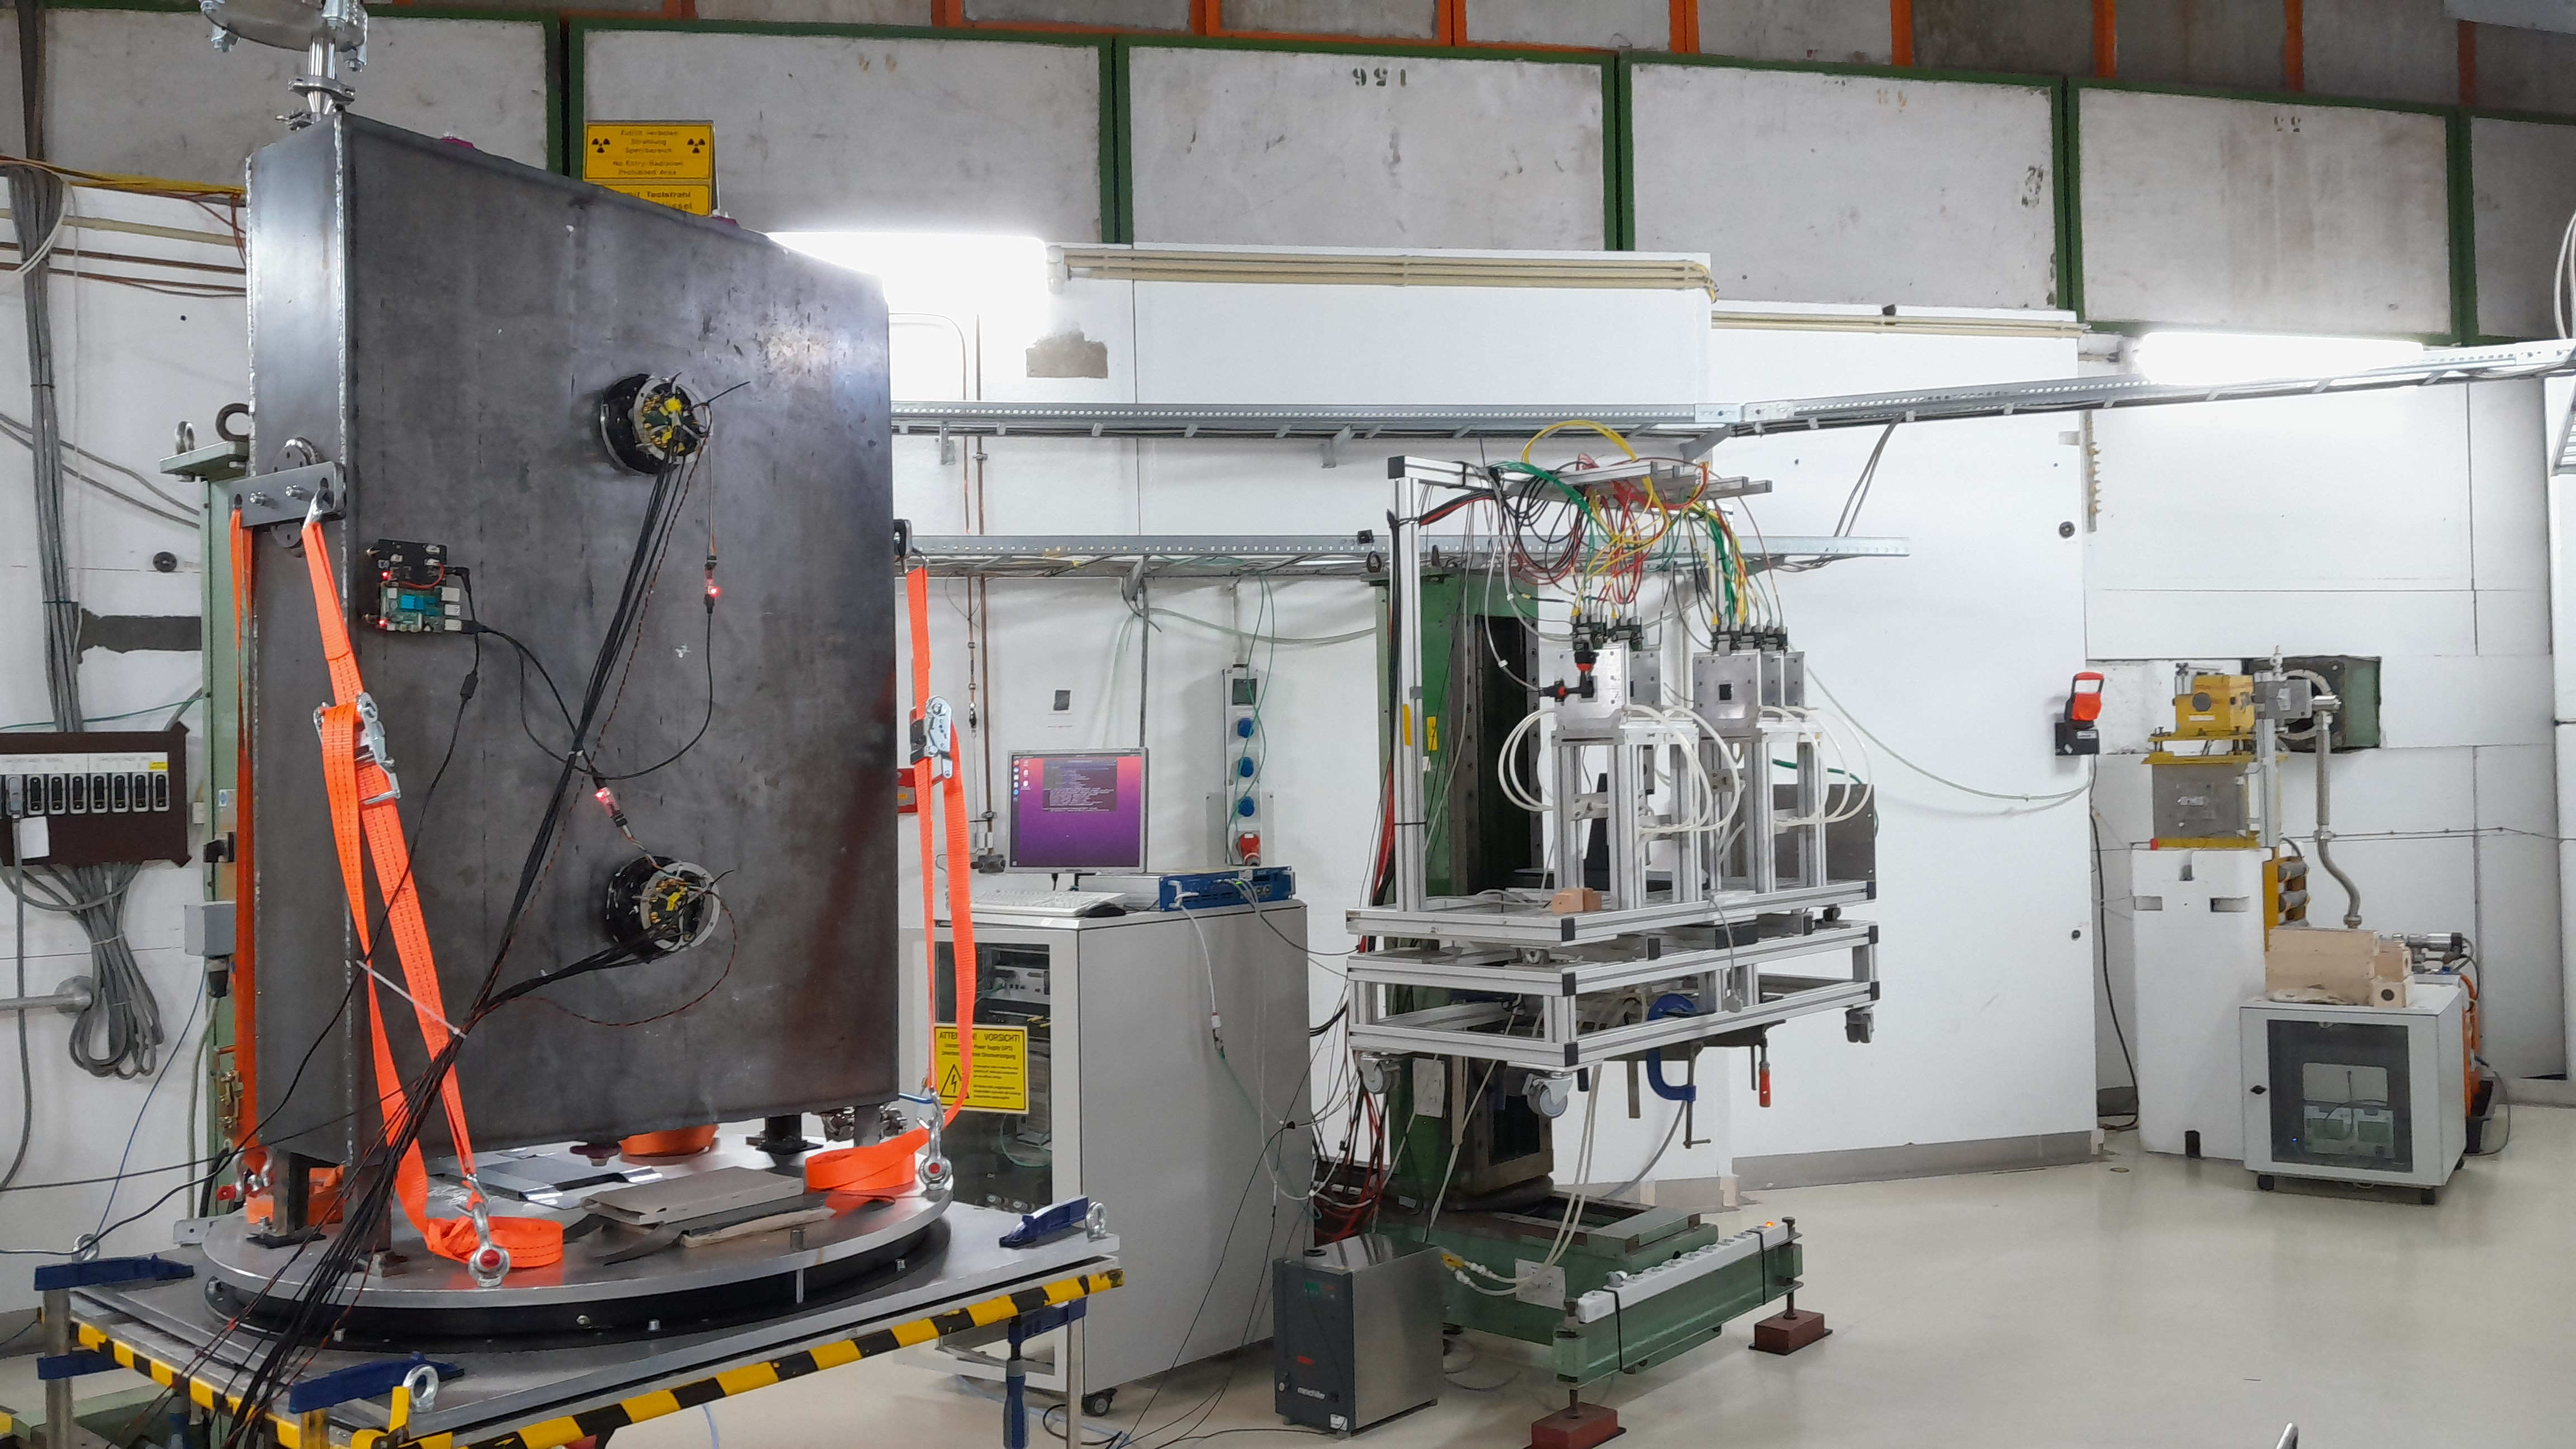
\includegraphics[width=1.\textwidth]{pictures/one_cell_testbeam}
	\caption[One Cell Prototype at the \ac{desy} testbeam]{Picture of the One Cell Prototype set up in the \ac{desy} testbeam area. The electron beam is coming from the right and is focused by a lead collimator. After the collimator the beam telescope consisting of four plastic scintillators and \ac{pmt} is placed as a trigger for the data aquisition. Next to the beam telescope is the One Cell Prototype. It is placed on a rotatry table and a \ac{desy} table for left-right and up-down movement. The power supplies and the digitizer are not shown in this picture.}
	\label{fig:one_cell_testbeam}
\end{figure}

During the testbeam the \acp{wom} were read out with Hamamatsu \acp{sipm}, except for a few measurements using the SensL \acp{sipm} for comparisson.
The optical coupling between the \acp{wom} and the \acp{sipm} was done with silicon pads.
Test measurements were performed using optical gel instead of the silicon pad, since the optical gel was used in previous testbeams.
The \ac{sipm} signals were amplified and shaped by \ac{emusic} \acp{asic} with \ac{emusic} boards.
The \ac{emusic} configuration used for most of the measurements is shown in the appendix.
A few measurements used the settings but without the high transimpedance.
The low transimpedance was chosen espacially for a measurement where the electron beam was shot directly through the lower \ac{wom} since the output of the \ac{emusic} saturated with the high transimpedance setting.
The digitization was done by a 64 channel WaveCatcher.
It is a \SI{12}{\bit} digitizer with a sampling frequency of up to \SI{3.2}{\giga\sample\per\second} and a dynamic range of \SI{2.5}{\voltpp}.
The WaveCatcher also digitized the signals from the four beam telescope \acp{pmt} and triggered on a coincidence with a threshold of \SI{17}{\milli\volt}.
To supply the \ac{emusic} board with power, the same power supply used for the test measurements shown in the previous chapter is used.
For the power of the \acp{sipm} a custom, remote controllable power supply was build by Tim Molzberger in Freiburg.






After the performance of the \ac{daq} was tested at the testbeam for one week with particles of known energy and known direction of movement, the long term performance of the one cell prototype and the \ac{daq} needs to be investigated.
For this purpose, the one cell prototype is assembled at the University of Freiburg, where it is supposed to be taking continuously data for a year.
Here the majority of events will be caused by cosmic muons.
By adding plastic scintillators with \acp{pmt} above and below the detector, trigger the data aquisition on a coincidence to only measure events, where the partice passed vertically through the detector.
Also a way to calibrate the detector needs to be found.
